\documentclass[11pt,letterpaper]{article}
\usepackage{papernote}

\graphicspath{{huang2015_pigments/}}

% Five stacked panels must share one page: this width makes the total
% height fit the text block. Changing it will push a panel onto page 2.
\newlength{\panelw}
\setlength{\panelw}{4.28in}

\begin{document}

\papertitle{paper_title.png}

\begin{itemize}\setlength{\itemsep}{0.6em}
  \item \paperdoi{10.1371/journal.pone.0137029}
  \item Predictive relationships between hyperspectral regions and pigments is
        strong at leaf scale but decreases at canopy and landscape scales
        (Figure~\ref{fig:bands}).
  \item Provides a way to compute a ``meta-analysis'' $R^2$ over the 85 papers
        considered (Figure~\ref{fig:r2}).
\end{itemize}

\clearpage

\begin{figure}[H]
\centering
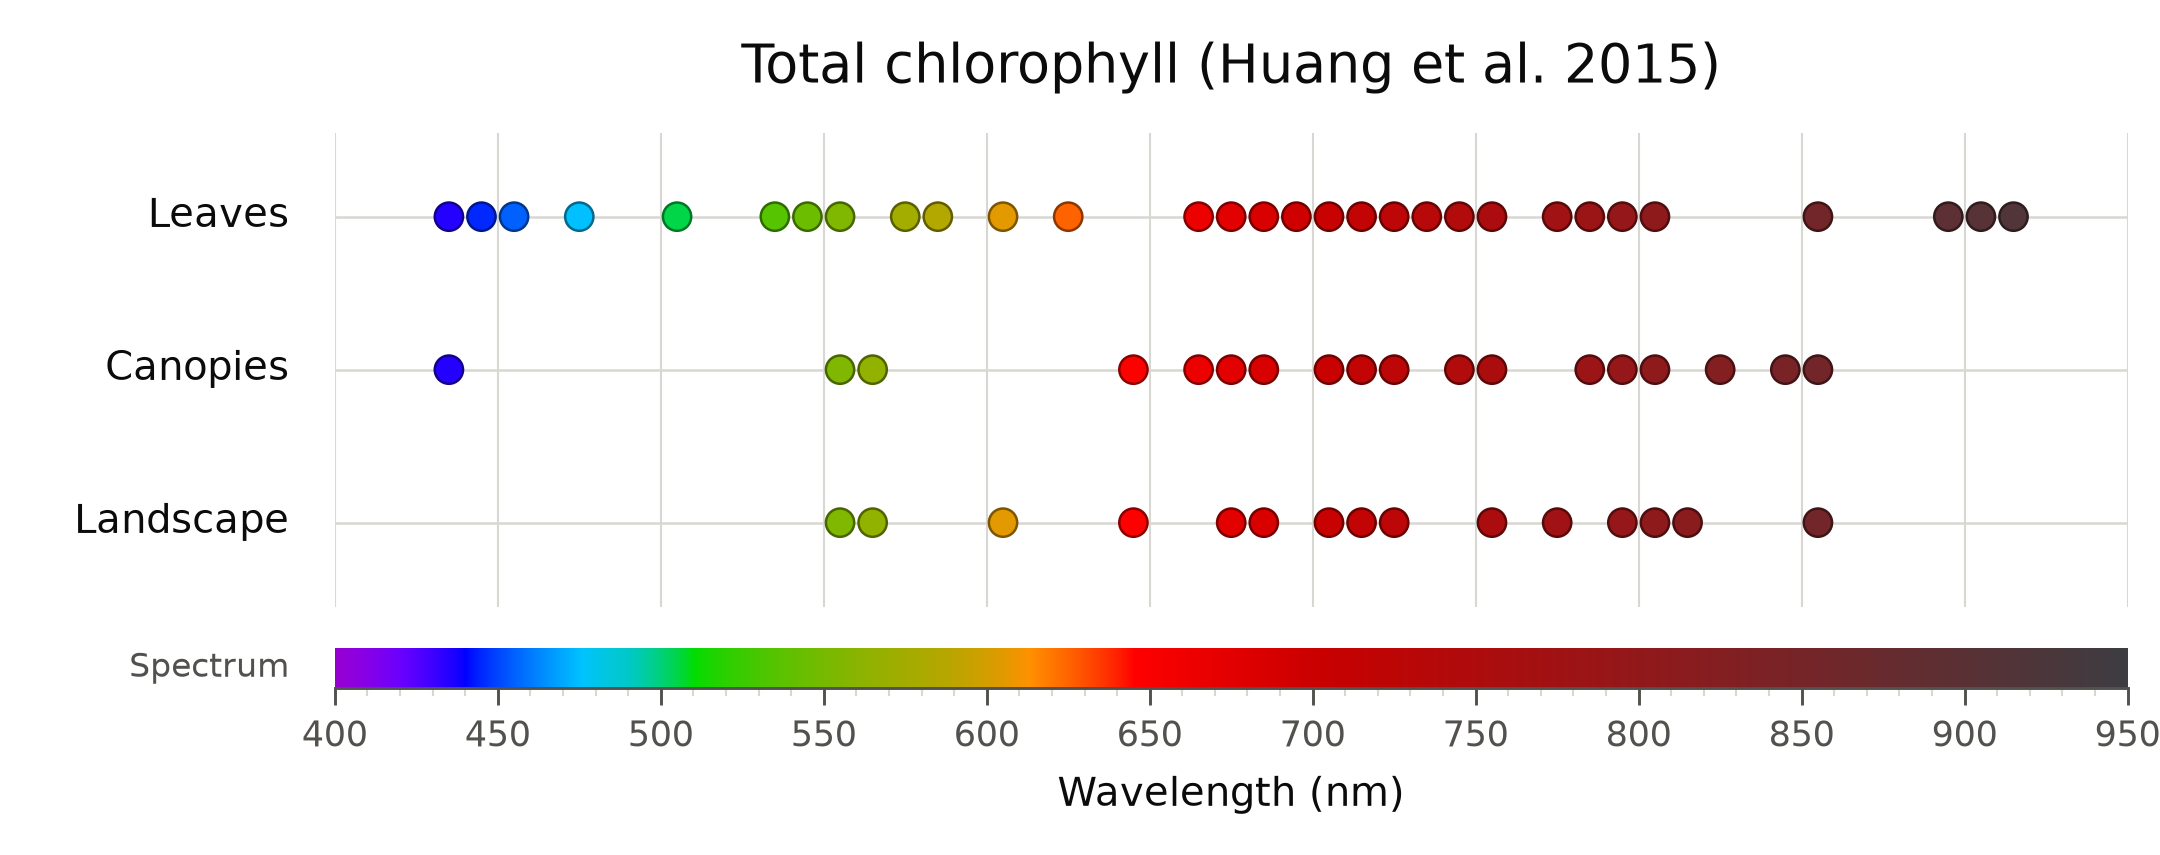
\includegraphics[width=\panelw]{huang2015_chlorophylls.png}\\[1pt]
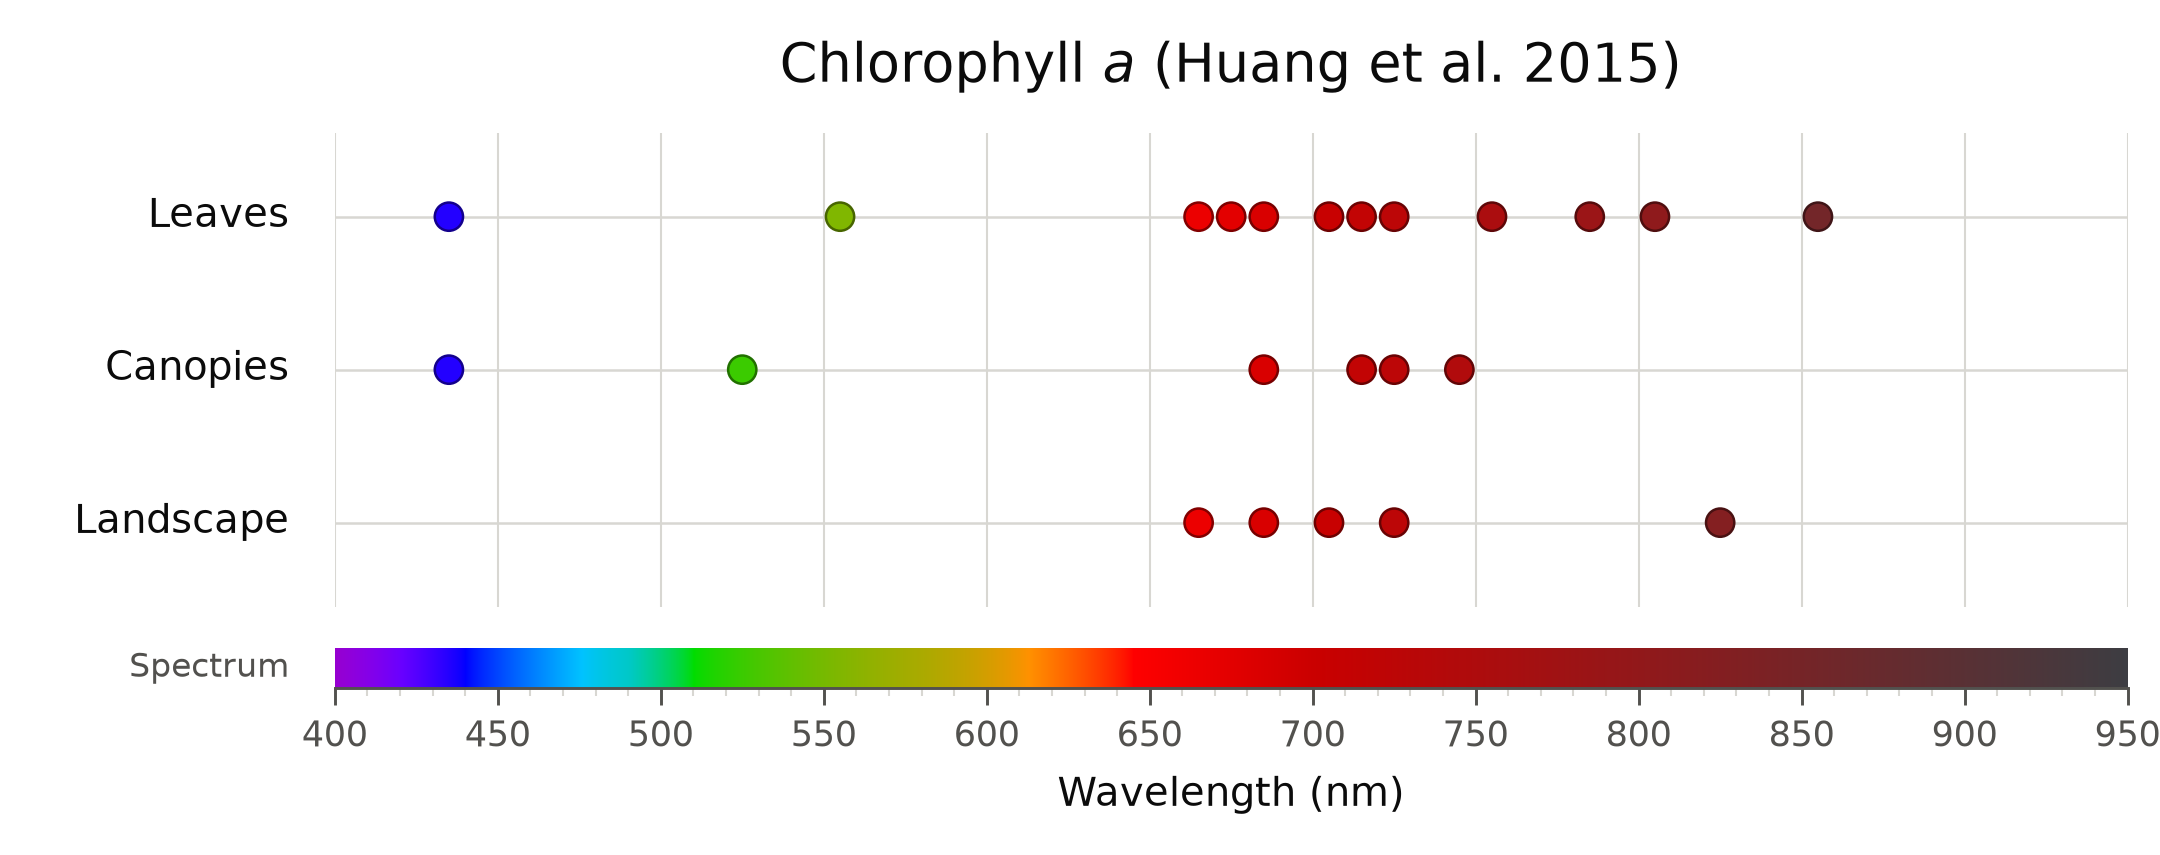
\includegraphics[width=\panelw]{huang2015_chlorophylla.png}\\[1pt]
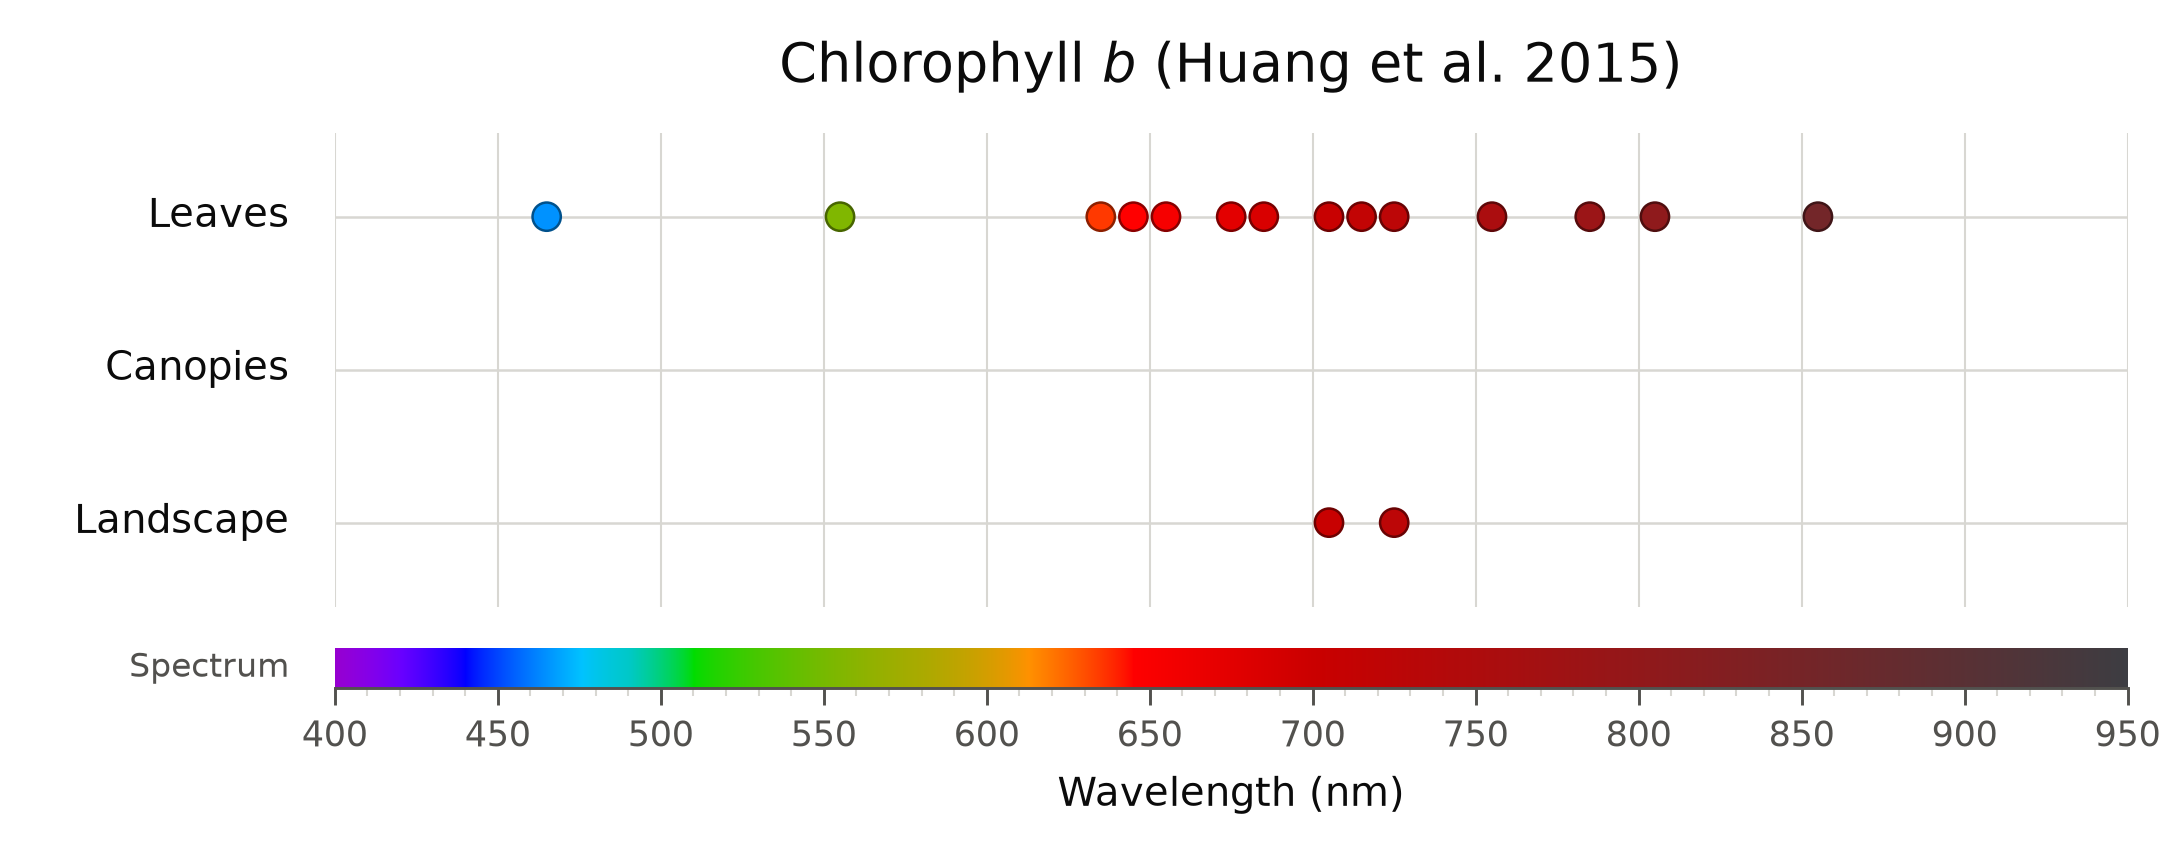
\includegraphics[width=\panelw]{huang2015_chlorophyllb.png}\\[1pt]
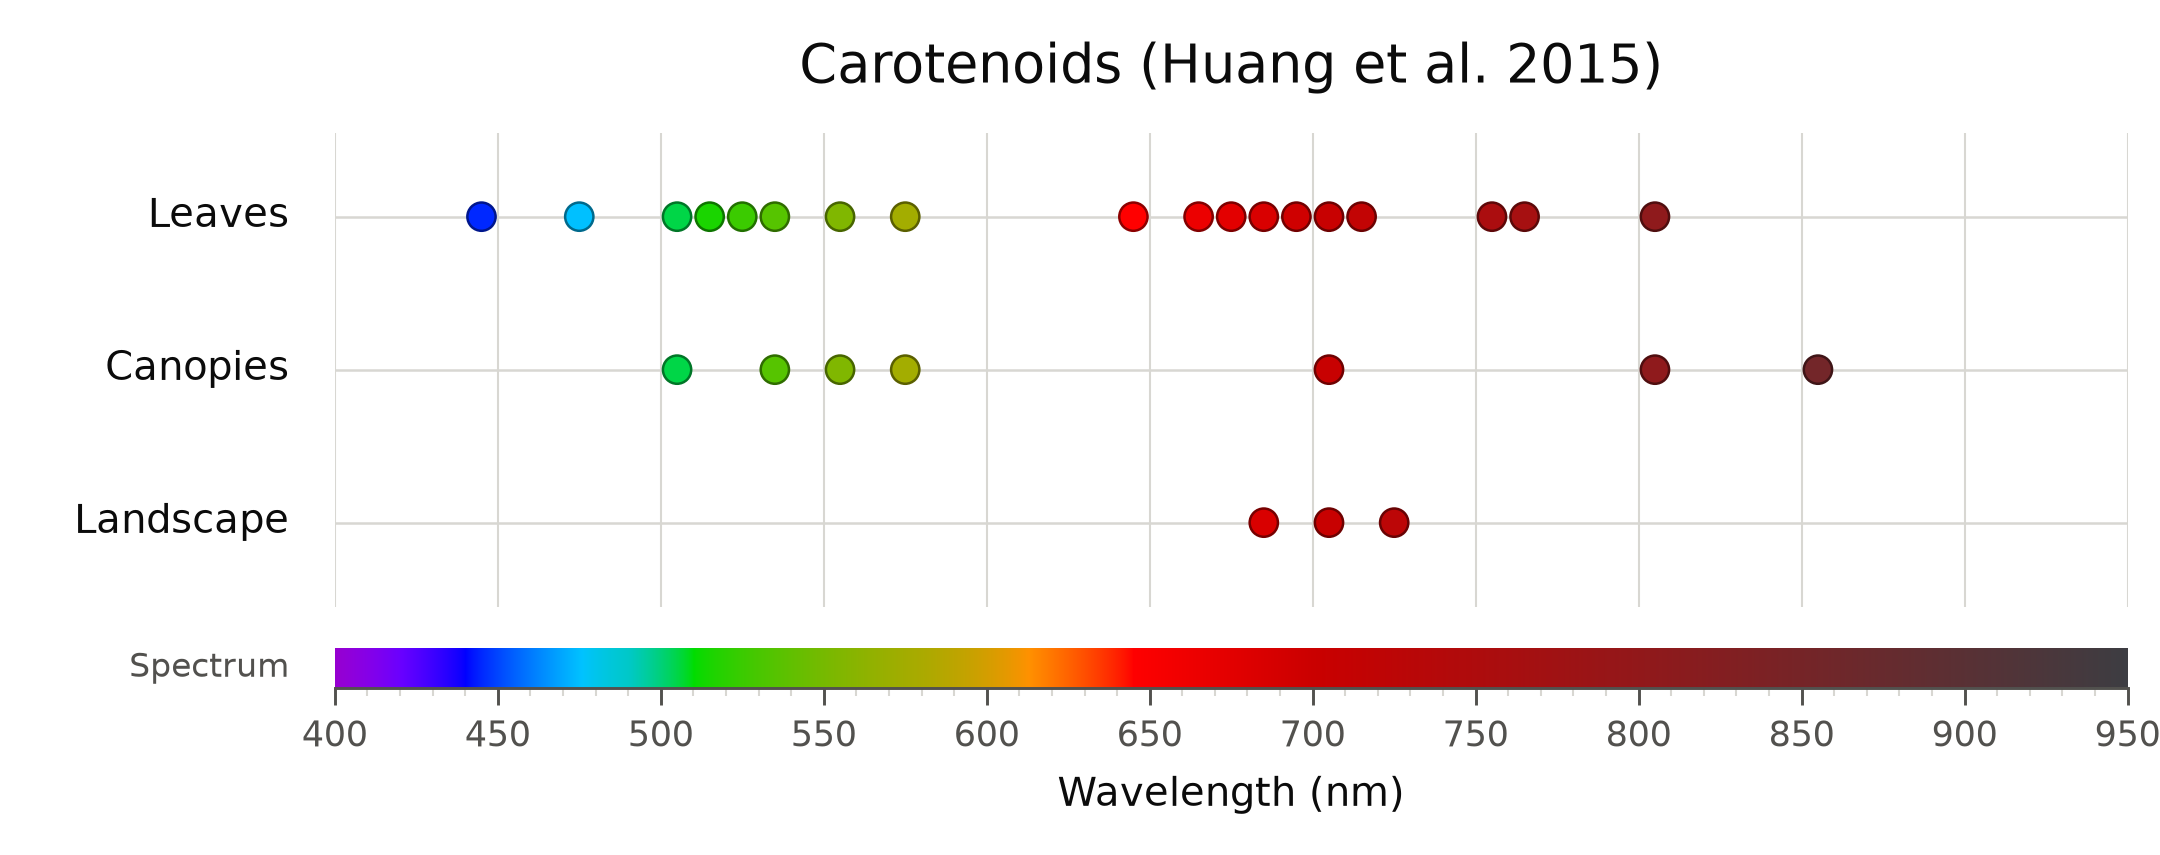
\includegraphics[width=\panelw]{huang2015_carotenoids.png}\\[1pt]
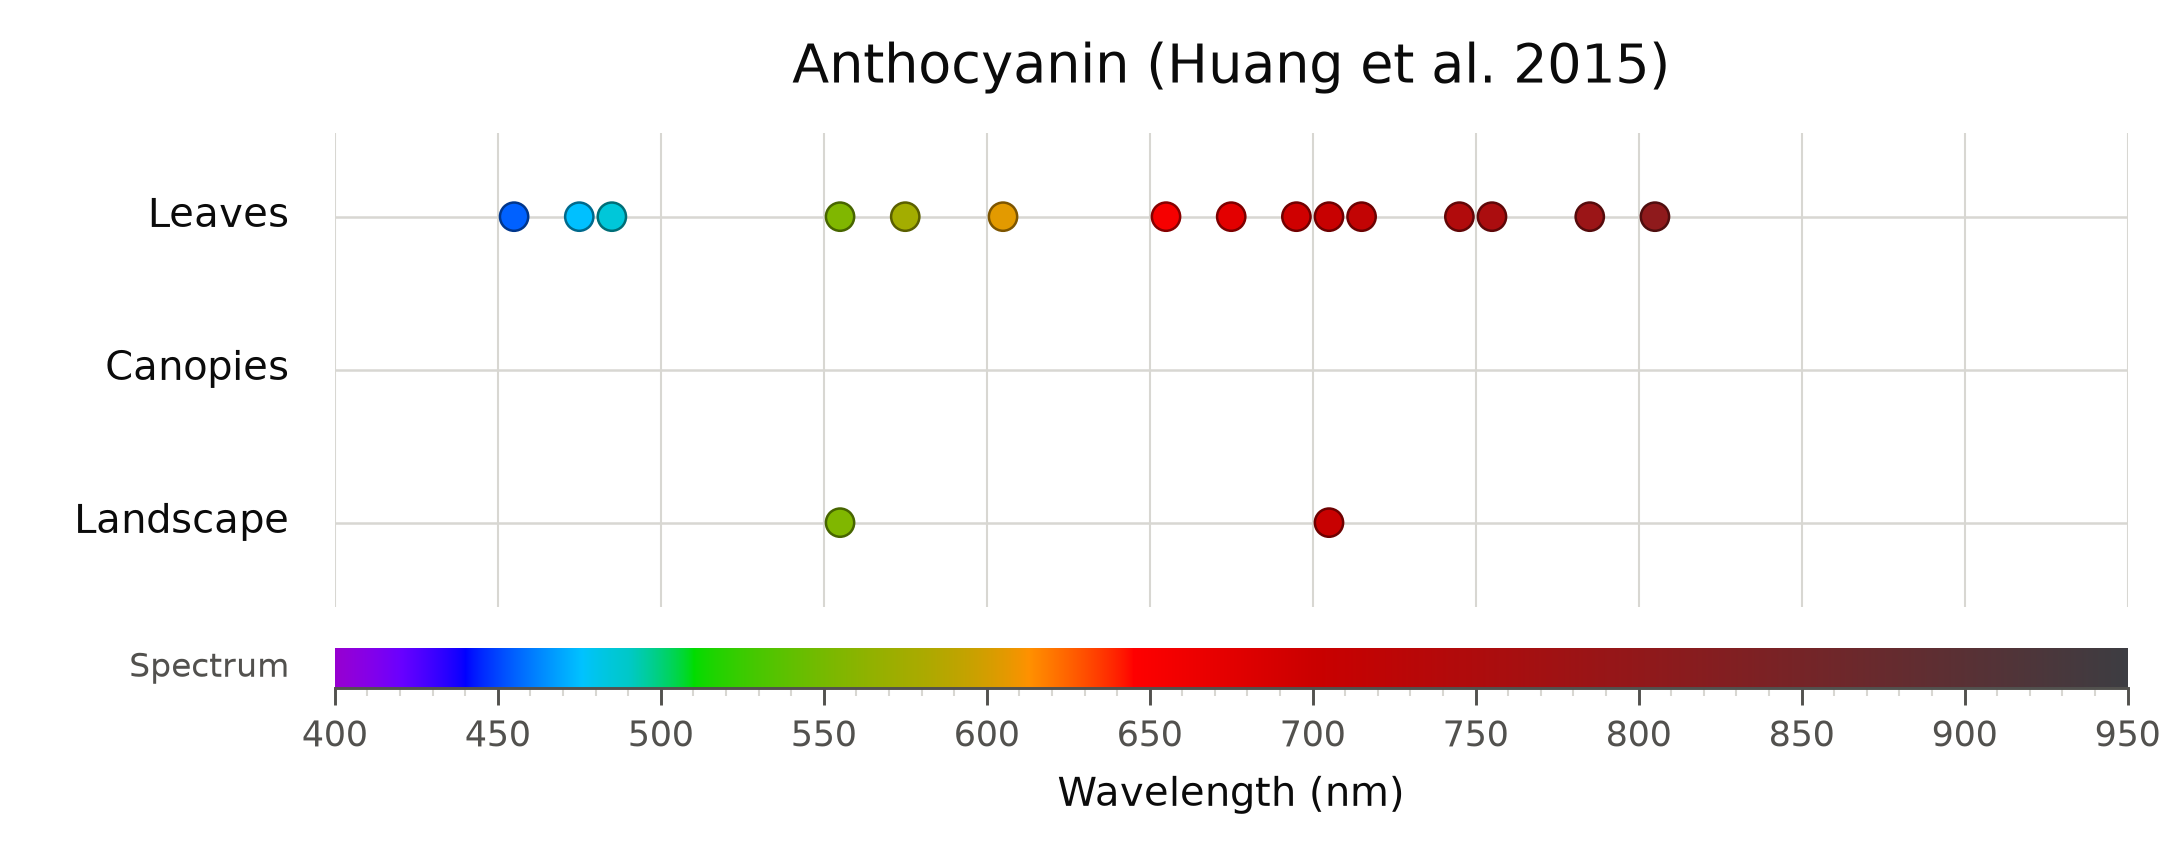
\includegraphics[width=\panelw]{huang2015_anthocyanin.png}
\caption{Meta-analysis of 85 studies. A dot denotes the 10\,nm bin being
reported as predictive in at least one study.}
\label{fig:bands}
\end{figure}

\clearpage

\begin{figure}[H]
\centering
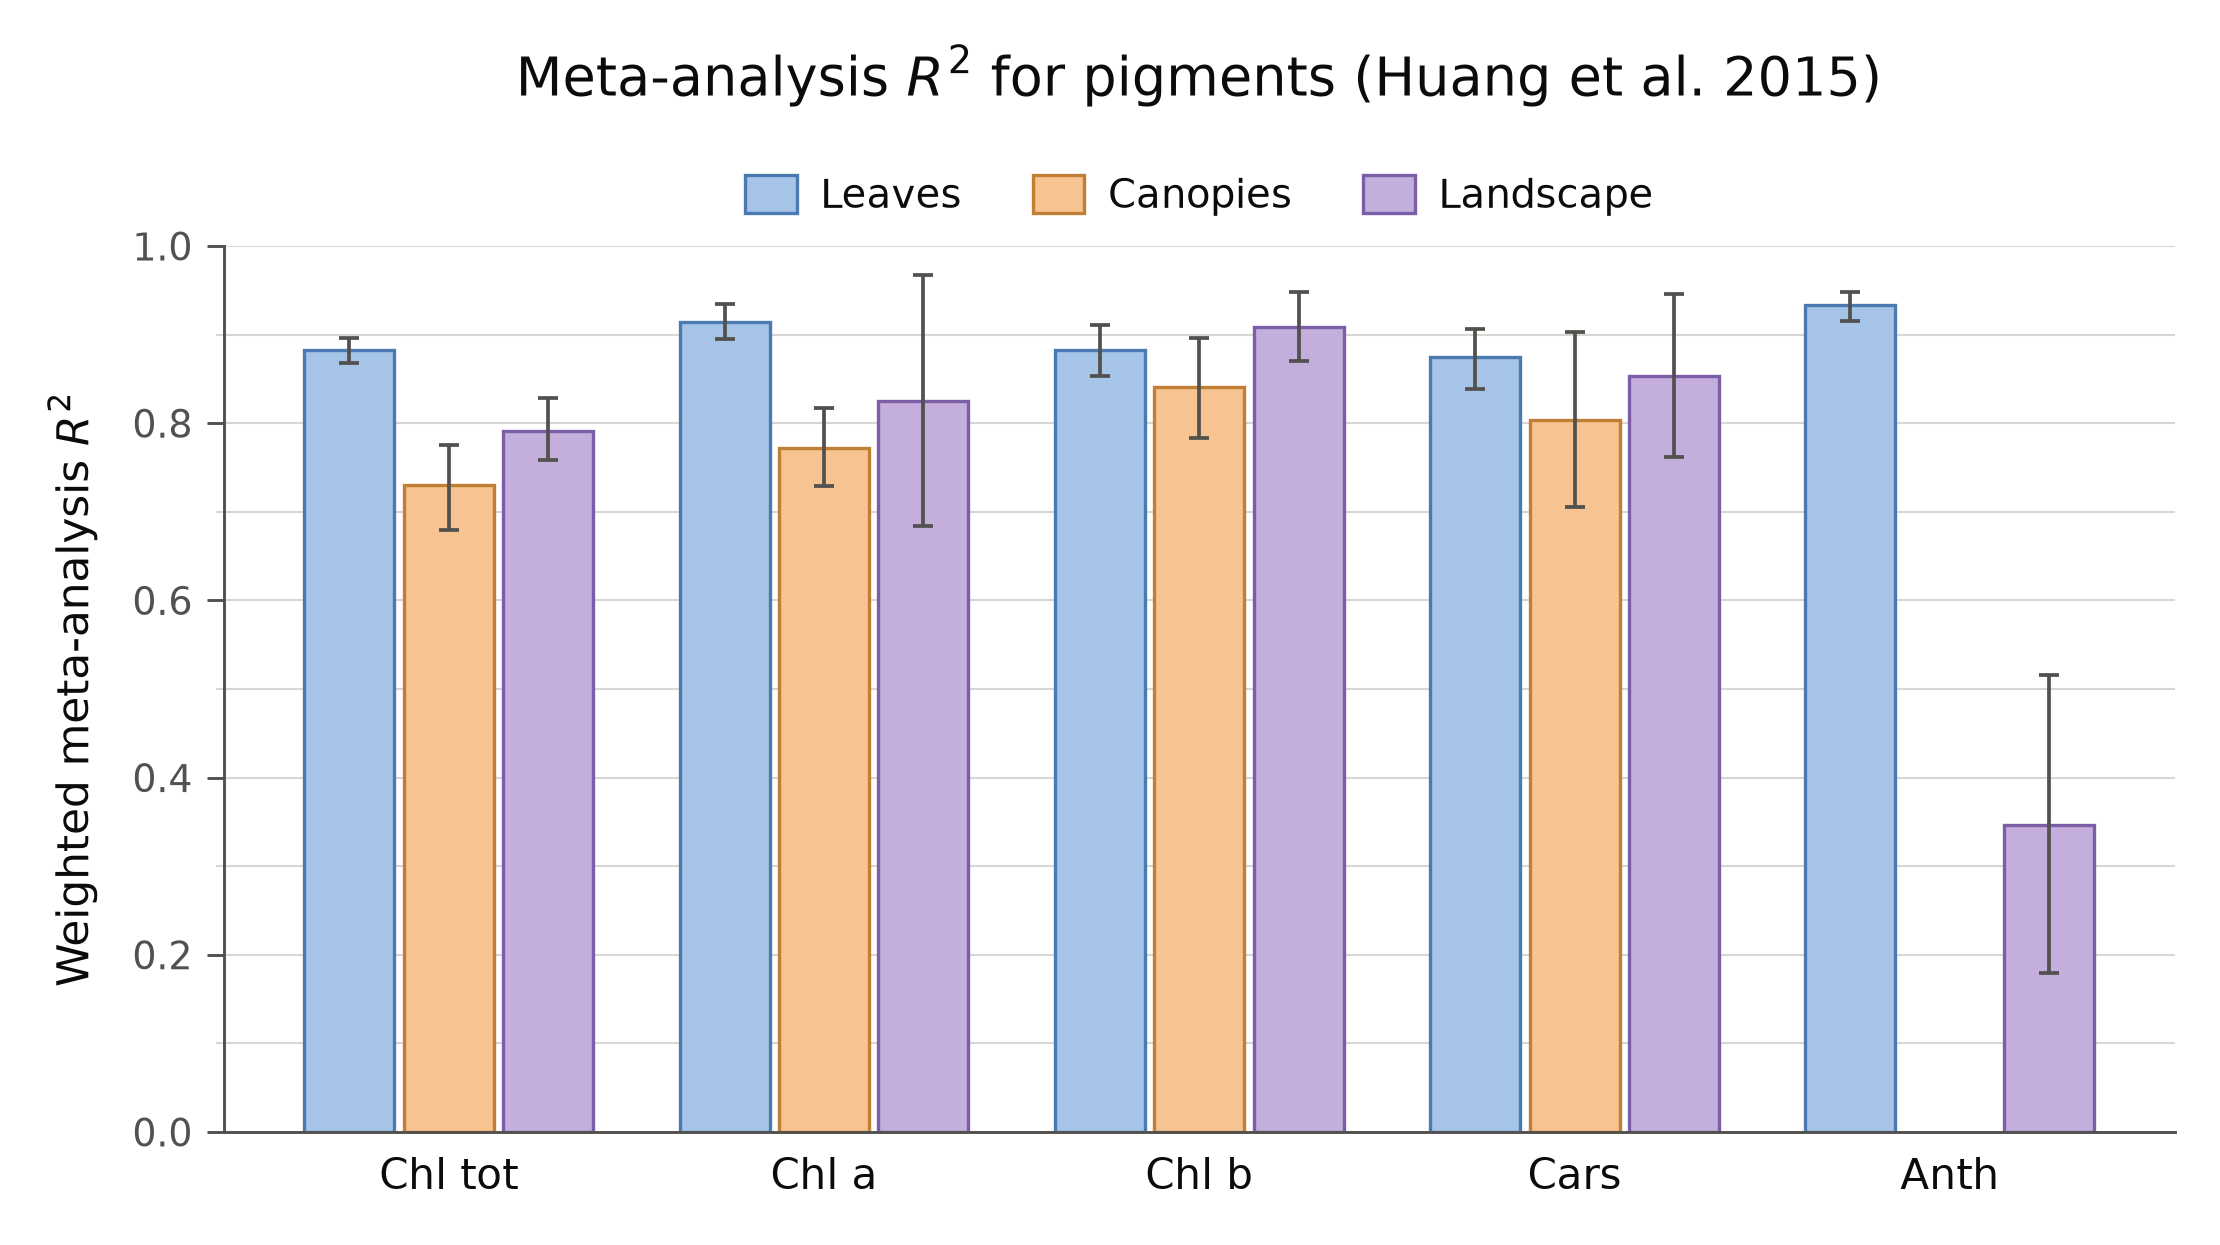
\includegraphics[width=0.96\textwidth]{meta_analysis_R2.png}
\caption{Weighted meta-analysis $R^2$ for each pigment at each observation
scale, based on meta-analysis of 85 studies.}
\label{fig:r2}
\end{figure}

\end{document}
